% \begin{savequote}[8cm]
% Alles Gescheite ist schon gedacht worden.\\
% Man muss nur versuchen, es noch einmal zu denken.

% All intelligent thoughts have already been thought;\\
% what is necessary is only to try to think them again.
%   \qauthor{--- Johann Wolfgang von Goethe \cite{von_goethe_wilhelm_1829}}
% \end{savequote}

\chapter{\label{ch:2-neutrinophysics}Neutrino physics}

\minitoc

This chapter includes a brief historical overview and a review of the introductory theoretical background of neutrino physics. In particular, the mechanism of neutrino oscillations will be described and several neutrino experimental anomalies will be analysed. The constraints and the hints for additional, non-weakly interacting neutrino states, will also be presented.

\section{Introduction}

Neutrino physics represents one of the most exciting areas of active research in particle physics. The history of the early days of particle physics shows that neutrinos have challenged physicists since the famous Pauli's letter to his fellow \emph{Radioactive Ladies and Gentlemen} \cite{Pauli:1930pc}. The continuous spectrum of the nuclear $\beta$-decay was then hypothesised by Fermi to be caused by the three-body process:
\begin{equation}
    n\rightarrow p + e^{-} + \bar{\nu}_{e},
\end{equation}
and mediated by a four-fermion interaction in the form of:
\begin{equation}
    \frac{G_{F}}{\sqrt{2}}(\bar{n}\Gamma_{N}p)(\bar{\nu}_{e}\Gamma_{L}e),
\end{equation}
where, in modern terms, $G_{F}$ is the Fermi constant and $\Gamma_{N,L}$ are a linear combination of the \emph{gamma matrices}. The Feynman diagram of the four-fermion approximation of $\beta$-decay is shown in Figure \ref{fig:fermibeta}.

\begin{figure}
    \centering
    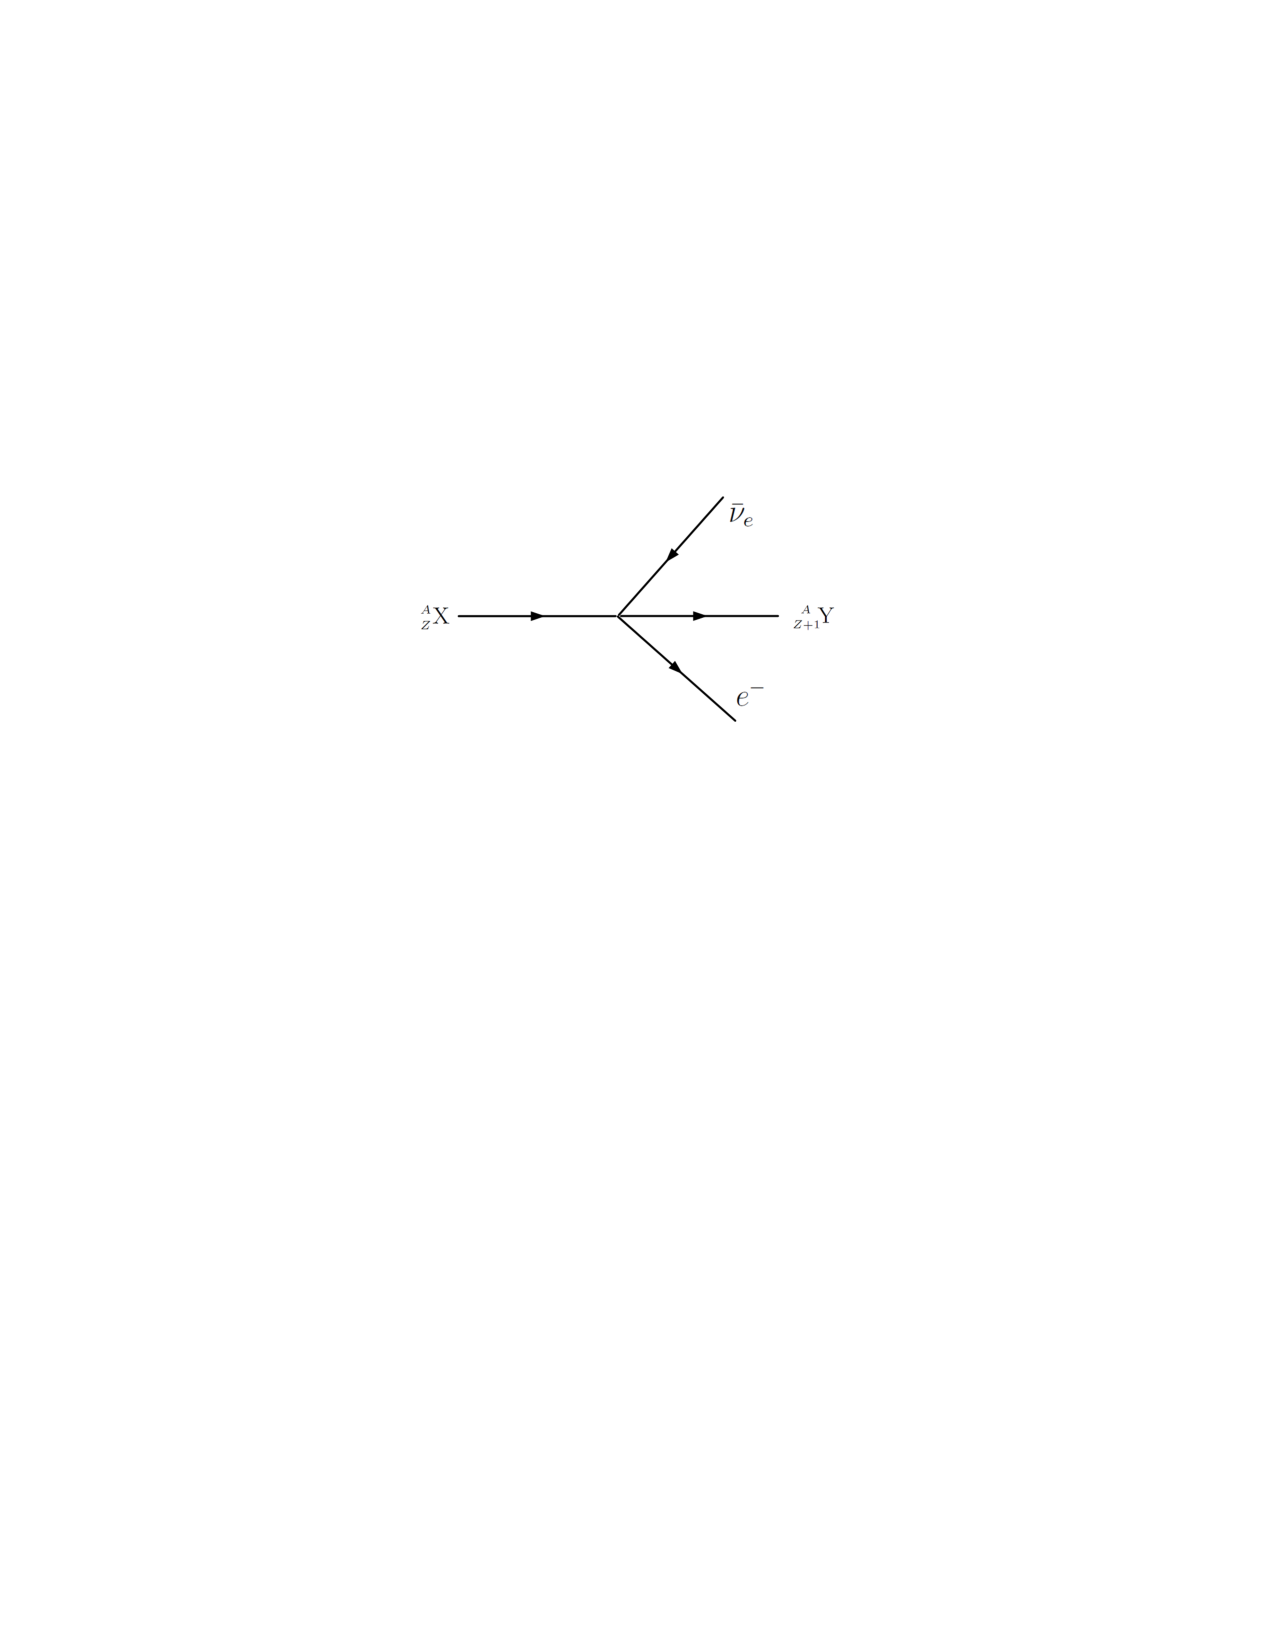
\includegraphics[width=0.7\linewidth]{figures/fermidecay.pdf}
    \caption{Feynman diagram of the $\beta$-decay of a $^{A}_{Z}X$ into a $^{A}_{Z+1}Y$ nucleus in the Fermi approximation.}
    \label{fig:fermibeta}
\end{figure}

This theory paved the way for the first experimental direct detection of neutrinos by Cowan and Reines in 1956 \cite{Cowan:1992xc}, which exploited the inverse $\beta$-decay process:
\begin{equation}
    \bar{\nu}_{e} + p \rightarrow e^{+} + n.
\end{equation}
The key detection technique, still used in modern reactor experiments, employed the detection of the $e^{+}e^{-}\rightarrow 2\gamma$ annihilation and a the $\gamma$ emitted by the recoiling neutron shortly afterwards. 

The leptonic current $\bar{\nu}_{e}\Gamma_{L}e$ was later verified to be left-handed in the form of $\gamma_{\mu}(1-\gamma_{5})$ ($V-A$). 
For massless neutrinos this allows to assign a left-handed (right-handed) helicity to neutrinos (anti-neutrinos), which was experimentally verified by Goldhaber in 1958 \cite{Goldhaber:1958nb}.

\section{Neutrino Oscillations Theory}
In the modern Standard Model of particle physics there are three flavours of (anti)neutrinos ($\nu_{e}$, $\nu_{\mu}$, $\nu_{\tau}$), each one paired to a charged (anti)lepton ($e$, $\mu$, $\tau$ respectively). 
However, if neutrinos have masses, it is possible to have three (or more) neutrino mass eigenstates ($\nu_{1}$, $\nu_{2}$, $\nu_{3}$, ...) analogues of the charged-lepton mass eigenstates. 
In this case, a neutrino produced as a flavour eigenstate would \emph{oscillate} through its path and change to another flavor eigenstate. This happens because the flavour eigenstate is a mixture of the three (or more) mass eigenstates, which travel with different wavelengths and create interference patterns. 

The oscillation probabilities can be easily derived in the case of two neutrino generations, which we follow for didactic reasons largely following the approach in \cite{deGouvea:2004gd}. The flavour eigenstates $\nu_{\alpha}, \nu_{\beta}$ can be expressed as a superposition of the two mass eigenstates $\nu_1$ and $\nu_2$ using the nominal rotation matrix $U$:
\begin{equation}
U = \begin{bmatrix}
    \cos\theta & -\sin\theta \\
    \cos\theta & \sin\theta
    \end{bmatrix}.
\end{equation}

The flavour neutrino $\nu_{\alpha}$ will then propagate as: 
\begin{equation}
    \ket{\nu_{\alpha}} = \cos\theta\ket{\nu_{1}}+\sin\theta\ket{\nu_{2}}
\end{equation}

The time evolution of this superposition can be written, in the plane-wave assumption, as:
\begin{equation}
    \ket{\nu(\vec{x},t)} = \cos\theta e^{-ip_{1}x}\ket{\nu_{1}}+\sin\theta e^{-ip_{1}x}\ket{\nu_{2}}.
\end{equation}
If the neutrino is ultra-relativistic the exponential argument becomes:
\begin{equation}
\begin{split}
    p_{i}x & = E_{i}t - \vec{p}_{i}\vec{x} \simeq (E_{i}-p_{z,i})L\\
           & = (E_{i}^2-|\vec{p}|^{2})/(E_{i}-p_{z,i})L\\
           & \simeq m_i^{2}/2E_{i}L \simeq m_i^{2}/2E L,
\end{split}
\end{equation}
and the oscillation probability of the neutrino with flavour $\alpha$ can be written as:
\begin{equation}
\begin{split}
    P_{\alpha\alpha} & = |\bra{\nu_{\alpha}}\ket{\nu(L)}|^2\\
                     & = 1 - \sin^2 2\theta \sin^2\left(\frac{\Delta m^{2}L}{4E}\right),\label{eq:prob}
\end{split}
\end{equation}
where $\Delta m^{2} \equiv m^2_2-m^2_1$ is the mass splitting. Eq. \eqref{eq:prob} shows that the amplitude of the oscillation is regulated by the rotation angle $\theta$, while its frequency depends on the mass splitting, at fixed energy $L/E$.

The $U$ matrix can be easily extended in the case of the three generations of neutrinos $\nu_{e}$, $\nu_{\mu}$, and $\nu_{\tau}$. In this case, the flavour eigenstates mixing is obtained from:
\begin{equation}
\begin{bmatrix}
\nu_{e}\\
\nu_{\mu}\\
\nu_{\tau}
\end{bmatrix}=
\begin{bmatrix} U_{e 1} & U_{e 2} & U_{e 3} \\ U_{\mu 1} & U_{\mu 2} & U_{\mu 3} \\ U_{\tau 1} & U_{\tau 2} & U_{\tau 3} 
\end{bmatrix} 
\begin{bmatrix} \nu_1 \\ \nu_2 \\ \nu_3 \end{bmatrix},
\end{equation}
where the rotation is given by the so-called Pontecorvo–Maki–Nakagawa–Sakata (PMNS) matrix. It is also possible to parametrise the $U$ matrix in the following useful way:
\begin{align} 
  U_{PMNS} = \begin{bmatrix} 1 & 0 & 0 \\ 0 & c_{23} & s_{23} \\ 0 & -s_{23} & c_{23} \end{bmatrix}
 \begin{bmatrix} c_{13} & 0 & s_{13}e^{-i\delta_{CP}} \\ 0 & 1 & 0 \\ -s_{13}e^{i\delta_{CP}} & 0 & c_{13} \end{bmatrix}
 \begin{bmatrix} c_{12} & s_{12} & 0 \\ -s_{12} & c_{12} & 0 \\ 0 & 0 & 1 \end{bmatrix},\label{eq:pmns}
\end{align}
where  $s_{ij}$ ($c_{ij}$) is an abbreviation for $\sin\theta_{ij}$ ($\cos\theta_{ij}$) and $\delta^{CP}$ is the CP-violating phase. The mixing angles $\theta_{12}$, $\theta_{13}$, and $\theta_{23}$ are defined by:
\begin{equation}
    \tan^2\theta_{12}\equiv\frac{|U_{e2}|^2}{|U_{e1}|^2},\quad
    \tan^2\theta_{23}\equiv\frac{|U_{\mu3}|^2}{|U_{\tau3}|^2},\quad
    \sin\theta_{13}\equiv U_{e3}e^{i\delta}.
\end{equation}

With three neutrino flavours the squared mass-splitting terms are $\Delta m_{12}^2$ and $\Delta m_{13}^2$. This cause a degeneracy in the ordering of three masses: it is possible to have $m_3 > m_2 > m_1$ (\emph{normal hierarchy}) or $m_3 > m_1 > m_2$ (\emph{inverted hierarchy}). Customarily, $\Delta m_{12}^2$ and $\Delta m_{13}^2$ are also called $(\Delta m^2)_{\mathrm{sol}}$ and $(\Delta m^2)_{\mathrm{atm}}$, respectively, since they are usually measured with "solar" and "atmospheric" neutrinos. The situation is illustrated in Figure \ref{fig:masshierarchy}, adapted from \cite{Cahn:2013taa}.

The mass splittings also determine the $L/E$ ratio at which the oscillation probability is maximised. In the assumption of two-neutrino oscillation, the oscillation frequency in eq. \eqref{eq:prob} becomes:
\begin{equation}
     \frac{\Delta m^{2}L}{4E} = 1.267\left(\frac{L}{\mathrm{km}}\right)\left(\frac{\Delta m^2}{\mathrm{eV}^2}\right)\left(\frac{\mathrm{GeV}}{E}\right),
\end{equation} 
which gives for $\theta_{12}$, $\theta_{13}$, and $\theta_{23}$ a maximum oscillation probability at $\approx 10^4$~km/GeV, $\approx 10^2$~km/GeV, and $\approx 10^2$~km/Gev, respectively. For this reason, $\theta_{12}$, $\theta_{13}$, and $\theta_{23}$ are also known as the \emph{solar}, \emph{reactor}, and \emph{atmospheric} mixing angles.

\begin{figure}
    \centering
    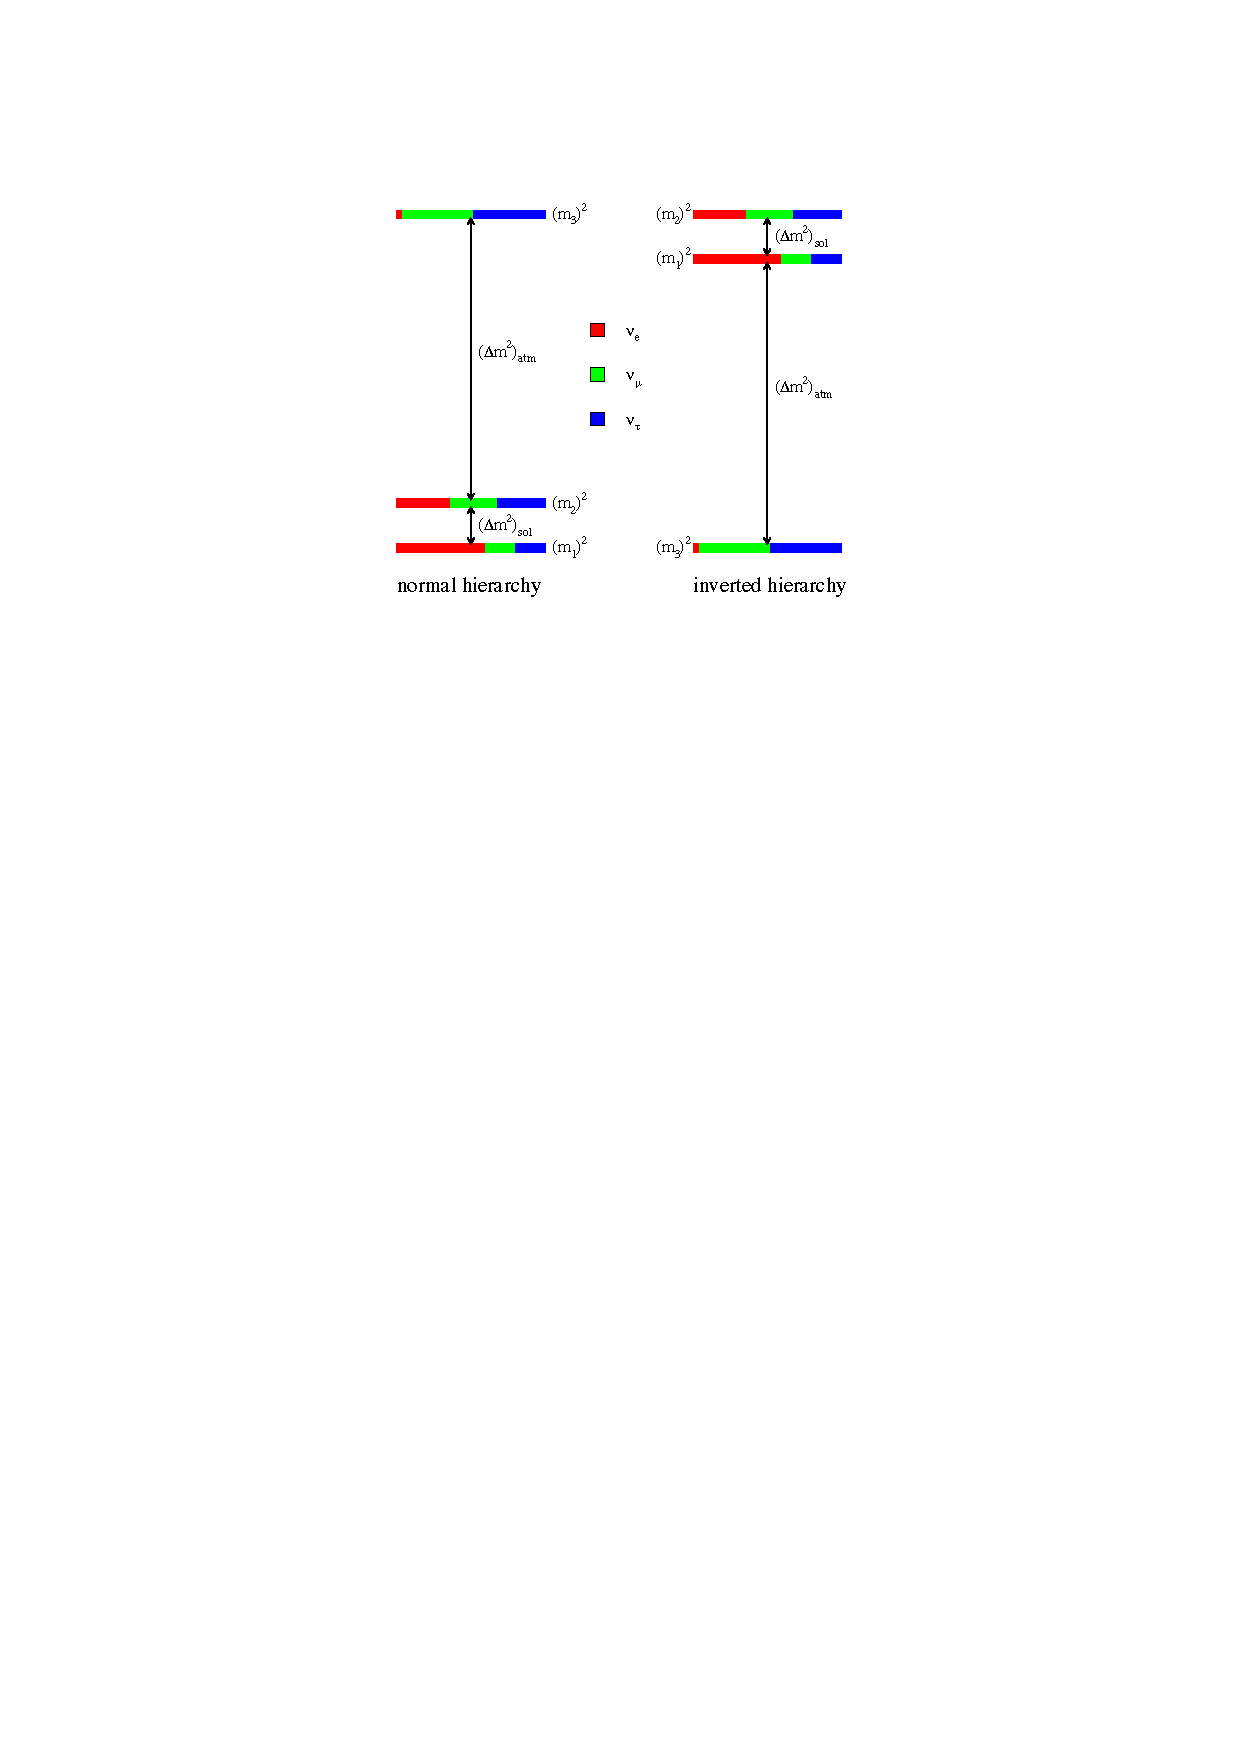
\includegraphics[width=0.75\linewidth]{figures/masshierarchy.pdf}
    \caption{Diagram of the normal and inverted hierarchies. The colours correspond to the fraction of each distinct flavor contained in the mass eigenstate.}
    \label{fig:masshierarchy}
\end{figure}

\section{Experimental Evidence of Neutrino Oscillation}
After the first direct detection of electron (anti)neutrinos by Cowan and Reines at the Savannah nuclear reactor, efforts were made in order to observe the other two neutrino flavours.
In 1962, Lederman and others \cite{PhysRevLett.9.36} first saw evidence of muon neutrinos interacting in the target and producing muons, while the DONUT collaboration finally observed the $\nu_{\tau}$ in 2001 \cite{Kodama:2000mp}.

However, the experiment by Ray Davis and others at Homestake observed a deficit in the number of solar neutrinos already in 1962, which was later confirmed by several other experiments. Evidence of atmospheric neutrino disappearance was provided by the Super-Kamiokande experiment \cite{Fukuda:1998mi}, while the SNO experiment proved the existence of neutrino oscillations by measuring both the solar $\nu_{e}$ flux and the total solar neutrino flux \cite{Ahmad:2002jz}. In honour of this discovery, the Nobel Prize in Physics 2015 was awarded to Takaaki Kajita (Super-Kamiokande) and Arthur B. McDonald (SNO). 

The propagation of neutrinos in the matter is also determined by the Mikheyev-Smirnov-Wolfenstein (MSW) effect: in presence of a high density of electrons, electron neutrinos experience a charged current coherent forward scattering. This cause the electron neutrinos to have a different effective mass when they propagate in a high-density medium, modifying the oscillation pattern. 

\begin{figure}[htbp]
    \centering
    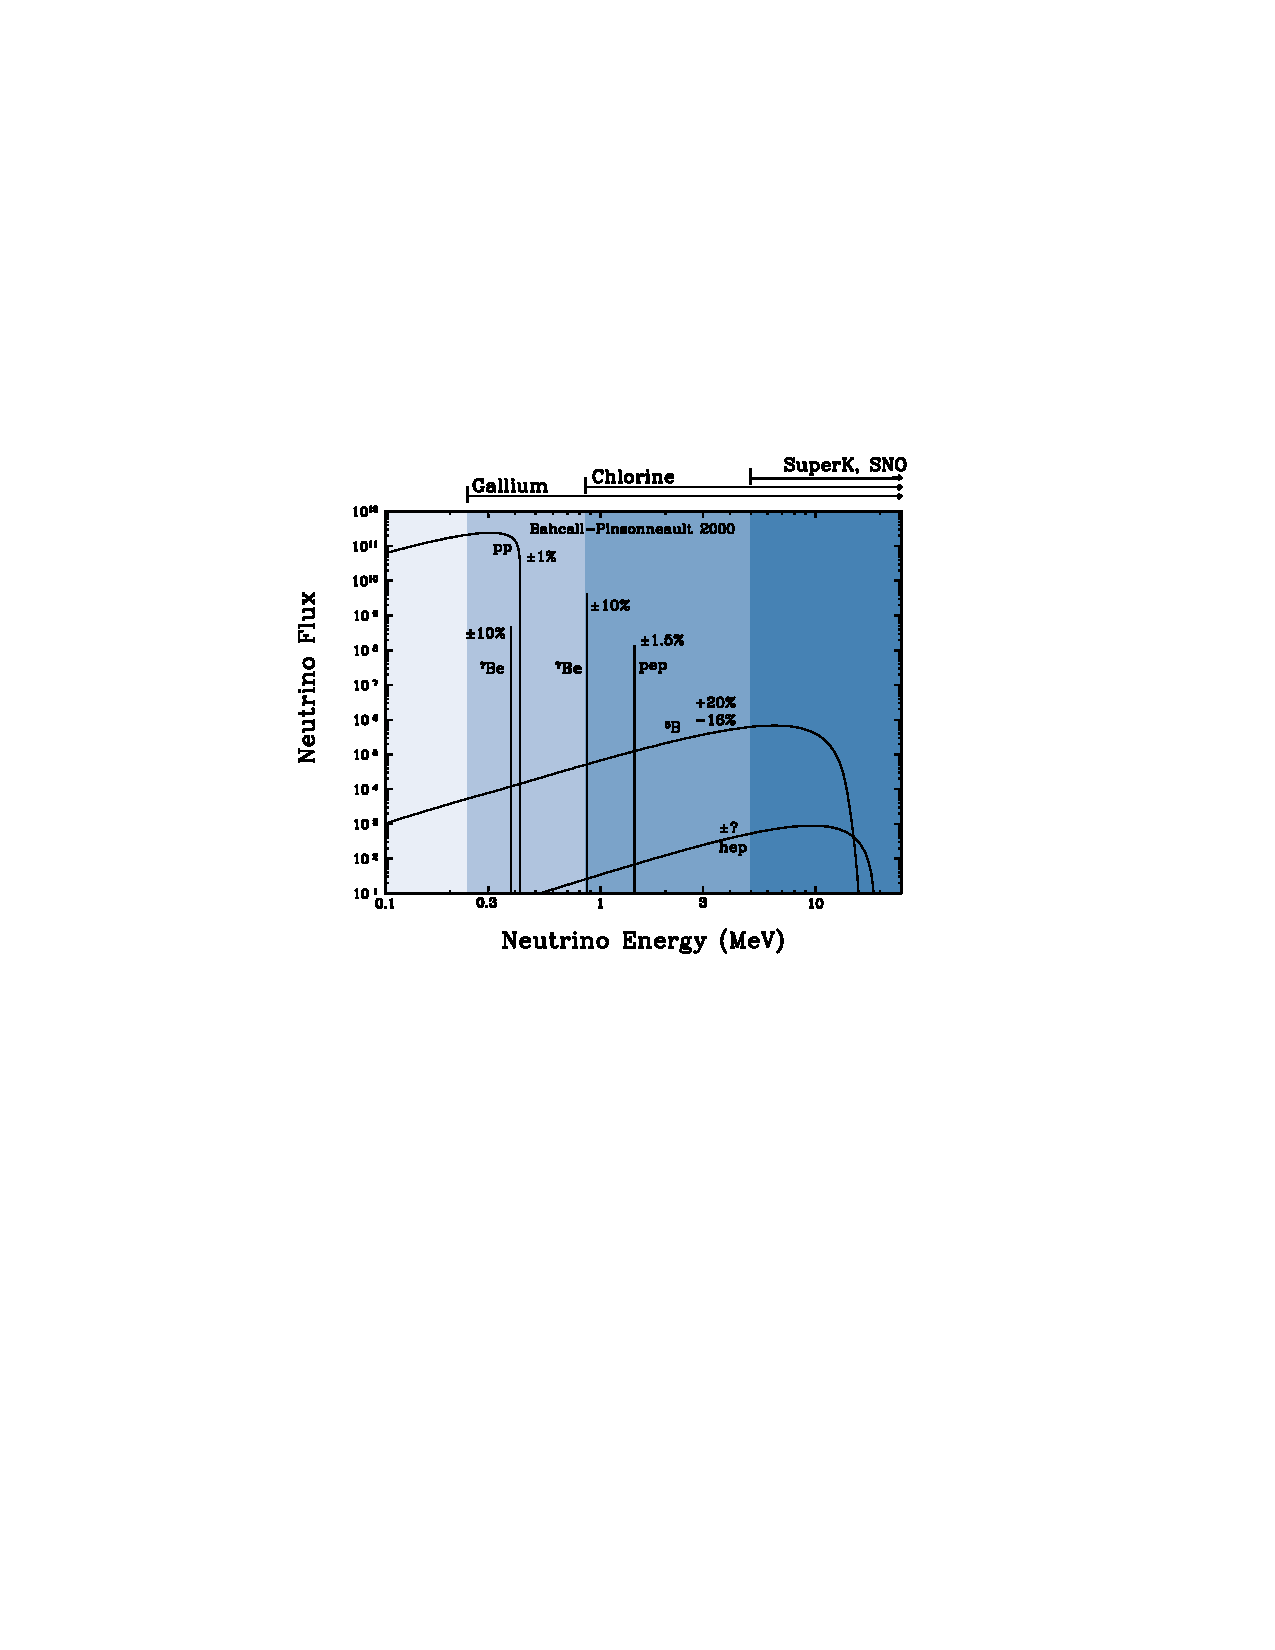
\includegraphics[width=0.75\linewidth]{figures/solar.pdf}
    \caption{The solar neutrino energy spectrum predicted by the solar standard model. Adapted from \cite{Bahcall:2000nu}.}
    \label{fig:solar}
\end{figure}

The MSW effect is particularly important to explain the solar neutrino flux (Figure \ref{fig:solar}). Assuming a very high electron density in the sun core and an exponentially decreasing abundance (which are both good approximations in the standard solar model), the probability to observe an electron neutrino when it reaches the Earth is $P_{ee} \approx \sin^2\theta$ for neutrinos above 2~MeV (where the matter effect dominates).



\begin{figure}[htbp]
    \centering
    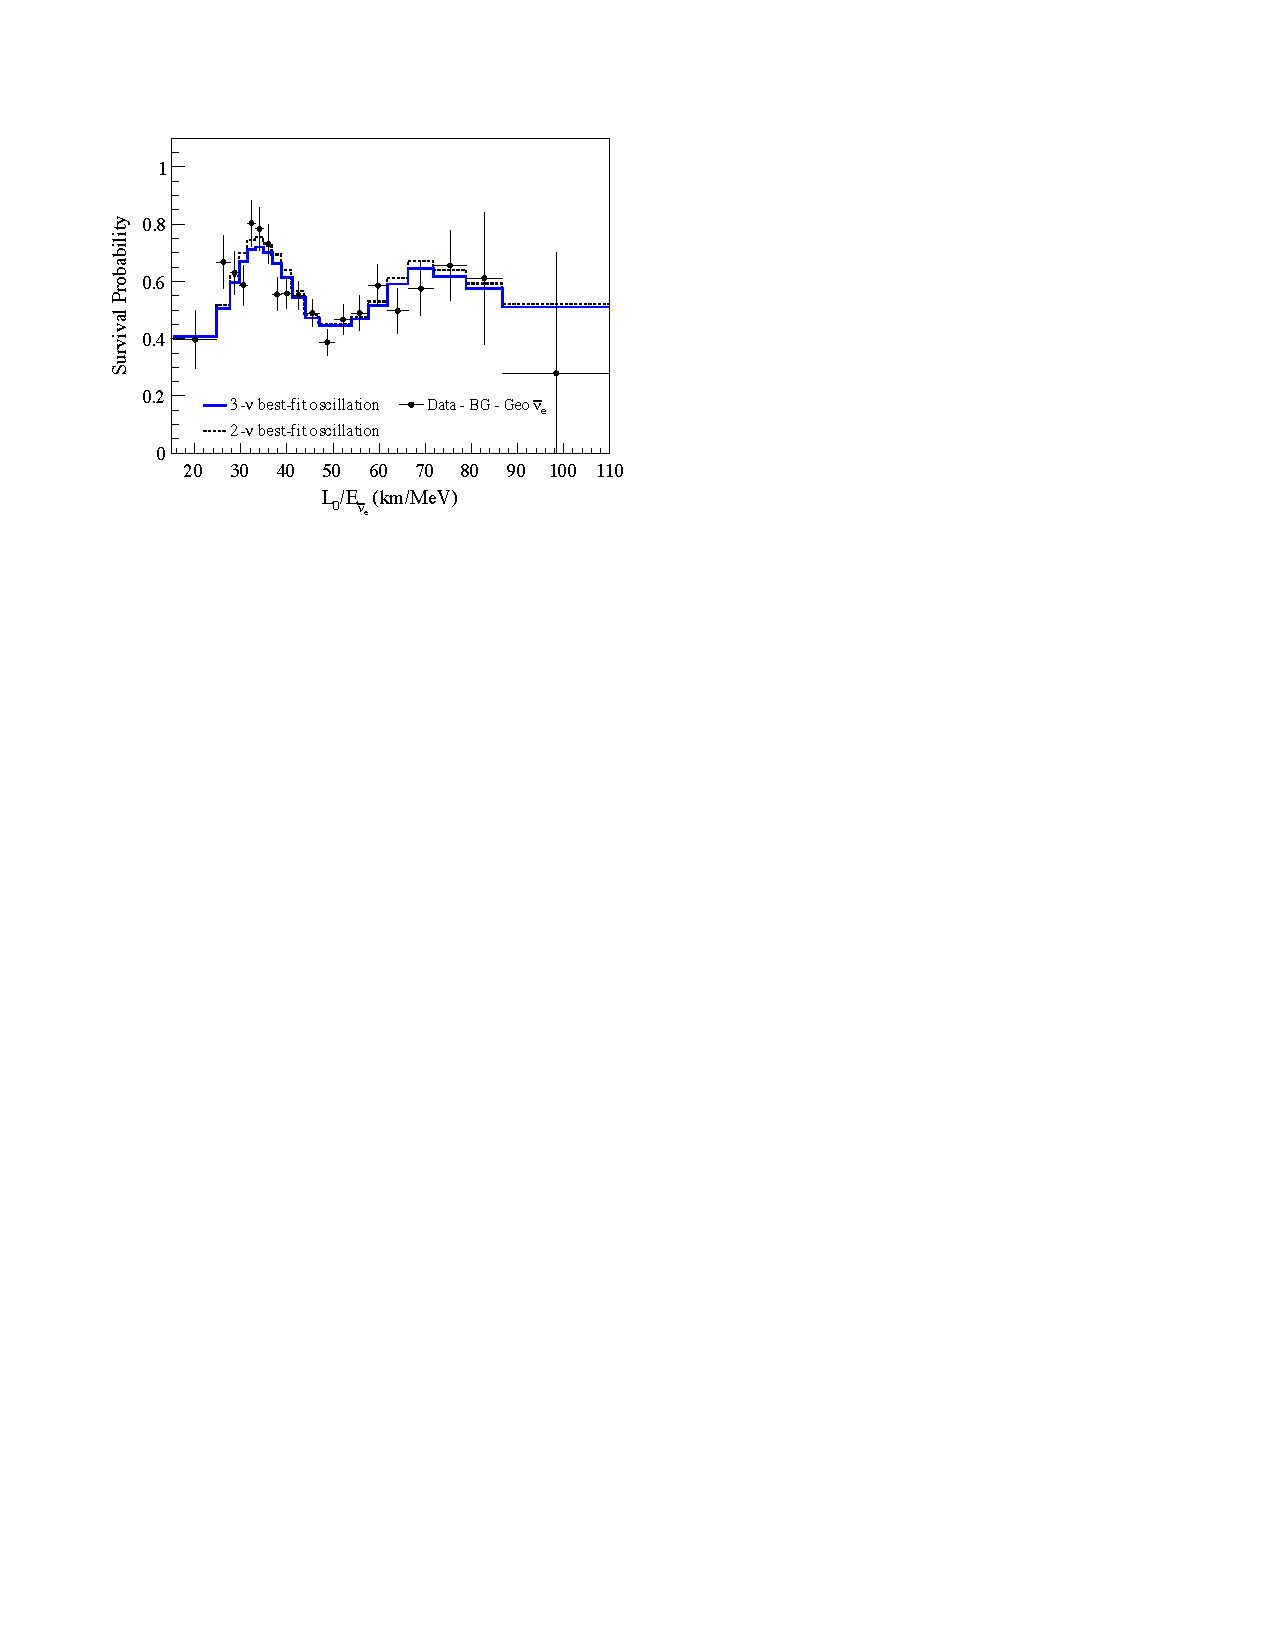
\includegraphics[width=0.75\linewidth]{figures/kamland.pdf}
    \caption{Ratio of the observed $\bar{\nu}_{e}$ spectrum to the expectation for no-oscillation versus $L_{0}/E$ for the KamLAND data. $L_{0} = 180$~km is the flux-weighted average reactor baseline. Adapted from \cite{Gando:2010aa}.}
    \label{fig:kamland}
\end{figure}

The KamLAND experiment finally spectacularly proved the oscillation pattern and the MSW model by measuring the reactor electron antineutrinos survival probability as a function of $L/E$, shown in Figure \ref{fig:kamland}. 

Less than 20 years after the definitive confirmation of neutrino oscillations, the mixing angles and the mass splittings are all known with a relative uncertainty smaller than 5\%. The least-known parameter in the PMNS matrix is the $\delta_{CP}$ phase, which, if different from $0^{\circ}$ (or from $180^{\circ}$), would imply CP-violation in the leptonic sector. This parameter can be measured only with appearance experiments, where it is possible to verify if
$P(\nu_{\alpha}\rightarrow\nu_{\beta}) \neq P(\bar{\nu}_{\alpha}\rightarrow\bar{\nu}_{\beta})$. Recent results from the T2K and NOVA experiments give a best fit of $\delta_{CP}/^{\circ}=215^{+40}_{-28}$ \cite{Esteban:2018azc}. A definitive measurement of the CP-violating phase would have far-reaching consequences in particle physics and cosmology, since it could explain the matter-antimatter asymmetry and provide an experimental basis for the leptogenesis model \cite{Fukugita:1986hr}.

The number of \emph{light} neutrino species (meaning $m_{\nu} < m_{Z}/2$) weakly interacting  was also determined by precision measurements of the $Z$ boson width at LEP as:
\begin{equation}
   N_{\nu} = \frac{\Gamma_{\mathrm{inv}}}{\Gamma_l}
   \left(\frac{\Gamma_{l}}{\Gamma_{\nu}}\right)_{\mathrm{SM}}=2.984\pm0.008.
\end{equation}

\section{Massive neutrinos in the Standard Model}
In the SM, quarks and leptons can be represented by a four-component Dirac spinor field $\psi_{D}$. This field can be decomposed into left-handed and right-handed two-component spinors with the chirality operators $\chi_{R} = (1+\gamma_5)\psi_D$ and $\chi_{L} = (1-\gamma_5)\psi_D$, respectively. The mass term for these spinors can be generated through the Higgs mechanism, which introduces a Dirac mass term in the Lagrangian:
\begin{equation}
    -\mathcal{L}_D = m_D\bar{\psi}_D\psi_D = m_D(\bar{\nu}_L\nu_R + \bar{\nu}_R\nu_L),
\end{equation}
which breaks chirality symmetry and makes helicity non-Lorentz-invariant.
This term can be applied also to neutrinos in an extension to the Standard Model. In this case, the neutrino would be a four-component massive Dirac spinor, just as any other fermion, with two components non-interacting.
However, the current upper limit on the sum of the neutrino masses is $\sum m_{\nu} < 0.23$~eV using cosmological constraints \cite{Ade:2015xua} and $\sum m_{\nu} < 2$~eV from $\beta$-decay experiments \cite{Otten:2008zz}. These results require a Yukawa coupling six orders of magnitude smaller than the electron one, which is not considered natural.

Another explanation for the neutrino masses would be the introduction of a Majorana mass term in the Lagrangian:
\begin{equation}
    -\mathcal{L}_M = m_M(\bar{\nu}_L\mathcal{C}\bar{\nu}^{T}_L+\nu_{L}\mathcal{C}\nu^T_L) = m_M(\bar{\nu}_M\nu_M),
\end{equation}
where $\nu_{M} \equiv \nu_L + \nu^c_R$ is the Majorana spinor and $\mathcal{C}$ is the charge-conjugation operator. An experimental evidence for Majorana neutrinos would be the observation of the $0\nu\beta\beta$ decay, where a $\nu_{e}$ is emitted and absorbed in the nucleus, producing two electrons and two protons in the final state. This process would also violate the lepton number with $\Delta L = 2$. In this case, the PMNS matrix in eq. \eqref{eq:pmns} acquires two extra Majorana phases in the form:
\begin{equation}
    U_{PMNS}^M = U_{PMNS} \begin{bmatrix}
    e^{i\alpha} & 0 & 0 \\
    0 & e^{i\beta} & 0 \\
    0 & 0 & 1
    \end{bmatrix}.
\end{equation}

A process which could explain the small masses of the neutrinos, compared to the other fermions, is the so-called \emph{seesaw} mechanism, which here we describe using the approach in \cite{Grossman:2003eb}. The addition of right-handed neutrinos to the SM allows to write the following neutrino mass matrix in $(\nu_L, \nu_R^c)$ basis:
\begin{equation}
    M = \begin{bmatrix}
    0 & m_D \\
    m_D & m_M
    \end{bmatrix},
\end{equation}
where $m_D$ is the Dirac mass term and $m_M$ is the Majorana mass term. For large values of $m_M$, this gives $m_{\nu_R}\approx m_M$ and $m_{\nu_L}\approx\frac{m_D^2}{m_M}$. With a value of $m_M$ at the GUT scale, this would \emph{naturally} give a small value for the neutrino masses.